In this chapter I will describe the architecture of the IoT platform, starting with a high-level glance -- the component diagram.

The smartwatch requires an application to propagate the data from the heart rate sensor to the mobile application through the \code{hr\_data} interface.
Once the raw data is received, it is combined with GPS data from the phone and forwarded through the \code{data\_access} interface to the IoT platform, where it gets processed and saved.
When the smartphone application requires it, it requests the processed data through the same interface and displays it.

\begin{figure}[h]
    \tmpframe{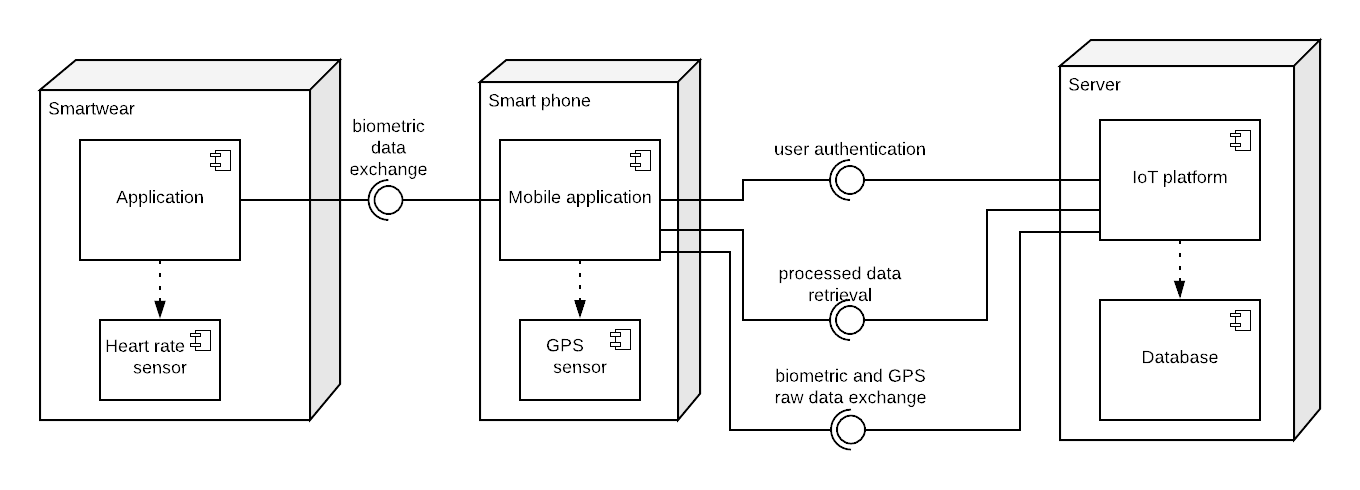
\includegraphics[width=\textwidth]{component.png}}
    \caption{Component diagram of the designed IoT solution.}
\end{figure}

Depending on the number and complexity of the features in the future, it is also possible to introduce a web client in order to make the smartphone APP lighter and easier to navigate.

The watch communicates with the phone application over Bluetooth, with the phone application acting as a server, waiting for the watch application to connect and send its data.
The phone application connects to the server using the phone's Internet connection.

\section{Smartwatch application}
Since the vendors of smartwatches generally use proprietary operating systems, every integrated smartwatch type needs an application of its own.
This is distributed together with the phone application.

Generally, it should be as light-weight as possible, to spare the limited battery resources.
Without any need for persistence, the application layer should collect the data from the heart rate sensors and regularly send them to the phone in batches.
The presentation layer displays data from the phone (such as instructions for a fitness test or navigation directions) received through the \code{directions} interface.
This is why it requires a bi-directional channel for Bluetooth communication.

\section{Smartphone application}
This phone app can easily follow the three-tier architecture: a persistent layer with a database for the user's planned hikes, a application layer for communication between the phone app, smartwatch app, and server, 


